% Options for packages loaded elsewhere
\PassOptionsToPackage{unicode}{hyperref}
\PassOptionsToPackage{hyphens}{url}
\PassOptionsToPackage{dvipsnames,svgnames,x11names}{xcolor}
%
\documentclass[
  letterpaper,
  DIV=11,
  numbers=noendperiod]{scrartcl}

\usepackage{amsmath,amssymb}
\usepackage{iftex}
\ifPDFTeX
  \usepackage[T1]{fontenc}
  \usepackage[utf8]{inputenc}
  \usepackage{textcomp} % provide euro and other symbols
\else % if luatex or xetex
  \usepackage{unicode-math}
  \defaultfontfeatures{Scale=MatchLowercase}
  \defaultfontfeatures[\rmfamily]{Ligatures=TeX,Scale=1}
\fi
\usepackage{lmodern}
\ifPDFTeX\else  
    % xetex/luatex font selection
\fi
% Use upquote if available, for straight quotes in verbatim environments
\IfFileExists{upquote.sty}{\usepackage{upquote}}{}
\IfFileExists{microtype.sty}{% use microtype if available
  \usepackage[]{microtype}
  \UseMicrotypeSet[protrusion]{basicmath} % disable protrusion for tt fonts
}{}
\makeatletter
\@ifundefined{KOMAClassName}{% if non-KOMA class
  \IfFileExists{parskip.sty}{%
    \usepackage{parskip}
  }{% else
    \setlength{\parindent}{0pt}
    \setlength{\parskip}{6pt plus 2pt minus 1pt}}
}{% if KOMA class
  \KOMAoptions{parskip=half}}
\makeatother
\usepackage{xcolor}
\setlength{\emergencystretch}{3em} % prevent overfull lines
\setcounter{secnumdepth}{-\maxdimen} % remove section numbering
% Make \paragraph and \subparagraph free-standing
\ifx\paragraph\undefined\else
  \let\oldparagraph\paragraph
  \renewcommand{\paragraph}[1]{\oldparagraph{#1}\mbox{}}
\fi
\ifx\subparagraph\undefined\else
  \let\oldsubparagraph\subparagraph
  \renewcommand{\subparagraph}[1]{\oldsubparagraph{#1}\mbox{}}
\fi


\providecommand{\tightlist}{%
  \setlength{\itemsep}{0pt}\setlength{\parskip}{0pt}}\usepackage{longtable,booktabs,array}
\usepackage{calc} % for calculating minipage widths
% Correct order of tables after \paragraph or \subparagraph
\usepackage{etoolbox}
\makeatletter
\patchcmd\longtable{\par}{\if@noskipsec\mbox{}\fi\par}{}{}
\makeatother
% Allow footnotes in longtable head/foot
\IfFileExists{footnotehyper.sty}{\usepackage{footnotehyper}}{\usepackage{footnote}}
\makesavenoteenv{longtable}
\usepackage{graphicx}
\makeatletter
\def\maxwidth{\ifdim\Gin@nat@width>\linewidth\linewidth\else\Gin@nat@width\fi}
\def\maxheight{\ifdim\Gin@nat@height>\textheight\textheight\else\Gin@nat@height\fi}
\makeatother
% Scale images if necessary, so that they will not overflow the page
% margins by default, and it is still possible to overwrite the defaults
% using explicit options in \includegraphics[width, height, ...]{}
\setkeys{Gin}{width=\maxwidth,height=\maxheight,keepaspectratio}
% Set default figure placement to htbp
\makeatletter
\def\fps@figure{htbp}
\makeatother

\KOMAoption{captions}{tableheading}
\makeatletter
\makeatother
\makeatletter
\makeatother
\makeatletter
\@ifpackageloaded{caption}{}{\usepackage{caption}}
\AtBeginDocument{%
\ifdefined\contentsname
  \renewcommand*\contentsname{Table of contents}
\else
  \newcommand\contentsname{Table of contents}
\fi
\ifdefined\listfigurename
  \renewcommand*\listfigurename{List of Figures}
\else
  \newcommand\listfigurename{List of Figures}
\fi
\ifdefined\listtablename
  \renewcommand*\listtablename{List of Tables}
\else
  \newcommand\listtablename{List of Tables}
\fi
\ifdefined\figurename
  \renewcommand*\figurename{Figure}
\else
  \newcommand\figurename{Figure}
\fi
\ifdefined\tablename
  \renewcommand*\tablename{Table}
\else
  \newcommand\tablename{Table}
\fi
}
\@ifpackageloaded{float}{}{\usepackage{float}}
\floatstyle{ruled}
\@ifundefined{c@chapter}{\newfloat{codelisting}{h}{lop}}{\newfloat{codelisting}{h}{lop}[chapter]}
\floatname{codelisting}{Listing}
\newcommand*\listoflistings{\listof{codelisting}{List of Listings}}
\makeatother
\makeatletter
\@ifpackageloaded{caption}{}{\usepackage{caption}}
\@ifpackageloaded{subcaption}{}{\usepackage{subcaption}}
\makeatother
\makeatletter
\@ifpackageloaded{tcolorbox}{}{\usepackage[skins,breakable]{tcolorbox}}
\makeatother
\makeatletter
\@ifundefined{shadecolor}{\definecolor{shadecolor}{rgb}{.97, .97, .97}}
\makeatother
\makeatletter
\makeatother
\makeatletter
\makeatother
\ifLuaTeX
  \usepackage{selnolig}  % disable illegal ligatures
\fi
\IfFileExists{bookmark.sty}{\usepackage{bookmark}}{\usepackage{hyperref}}
\IfFileExists{xurl.sty}{\usepackage{xurl}}{} % add URL line breaks if available
\urlstyle{same} % disable monospaced font for URLs
\hypersetup{
  colorlinks=true,
  linkcolor={blue},
  filecolor={Maroon},
  citecolor={Blue},
  urlcolor={Blue},
  pdfcreator={LaTeX via pandoc}}

\author{}
\date{}

\begin{document}
\ifdefined\Shaded\renewenvironment{Shaded}{\begin{tcolorbox}[interior hidden, borderline west={3pt}{0pt}{shadecolor}, sharp corners, boxrule=0pt, breakable, frame hidden, enhanced]}{\end{tcolorbox}}\fi

\hypertarget{experiment-18-cds1-repeat-2-2-fr}{%
\section{Experiment 18: CDS1 repeat \#2 (2
fr)}\label{experiment-18-cds1-repeat-2-2-fr}}

\textbf{Purpose}: To perform another repeat of CDS1 refolding with a
higher density. I think it worked better this time?

\textbf{Major results and comments:}

\begin{itemize}
\tightlist
\item
  Better density of molecules this time, managed to see a split peak
  distribution for last timepoint.
\item
  Need to perform final third repeat to see whether this or the other
  repeat is more true to what's really going on.
\end{itemize}

\textbf{Buffers used}:

\begin{itemize}
\tightlist
\item
  2x TROLOX buffer was made up in 2x refolding buffer (100 mM HEPES, 100
  mM KCL, 10 mM MgCl2, 2 mM DTT, 0.05\% T20 (pH 7.5)).
\item
  FlucCDS1 was unfolded by flowing in chemical denaturant (4 M GdHCl, 50
  mM HEPES, 50 mM KCl, 5 mM MgCl2, 0.05\% (v/v) T20)
\end{itemize}

\textbf{Concentration of proteins and stock origin}:

\begin{itemize}
\tightlist
\item
  3 uM A8 (127 uM stock origin- Shannon)
\item
  2 uM A2 (45 uM stock origin - Shannon)
\item
  0.5 Hsp110 (36.9 uM stock origin - Nicola)
\item
  Fluc flowed on at 50 pM concentration for immobilisation.
\end{itemize}

\textbf{Instrument/techniques/imaging settings:} 532 laser imaging
exposure = 0.2

532 nm laser = 1.6 ND

647 laser imaging exposure = 0.2

647 nm laser = 1.0 ND

\textbf{Setup and workflow:}

\begin{itemize}
\tightlist
\item
  CDS1 was immobilised at 5 nM concentration to achieve a high enough
  density for imaging. Could have pushed it up to 6 nM potentially,
  still not amazing density of molecule count.
\end{itemize}

\textbf{Data:}

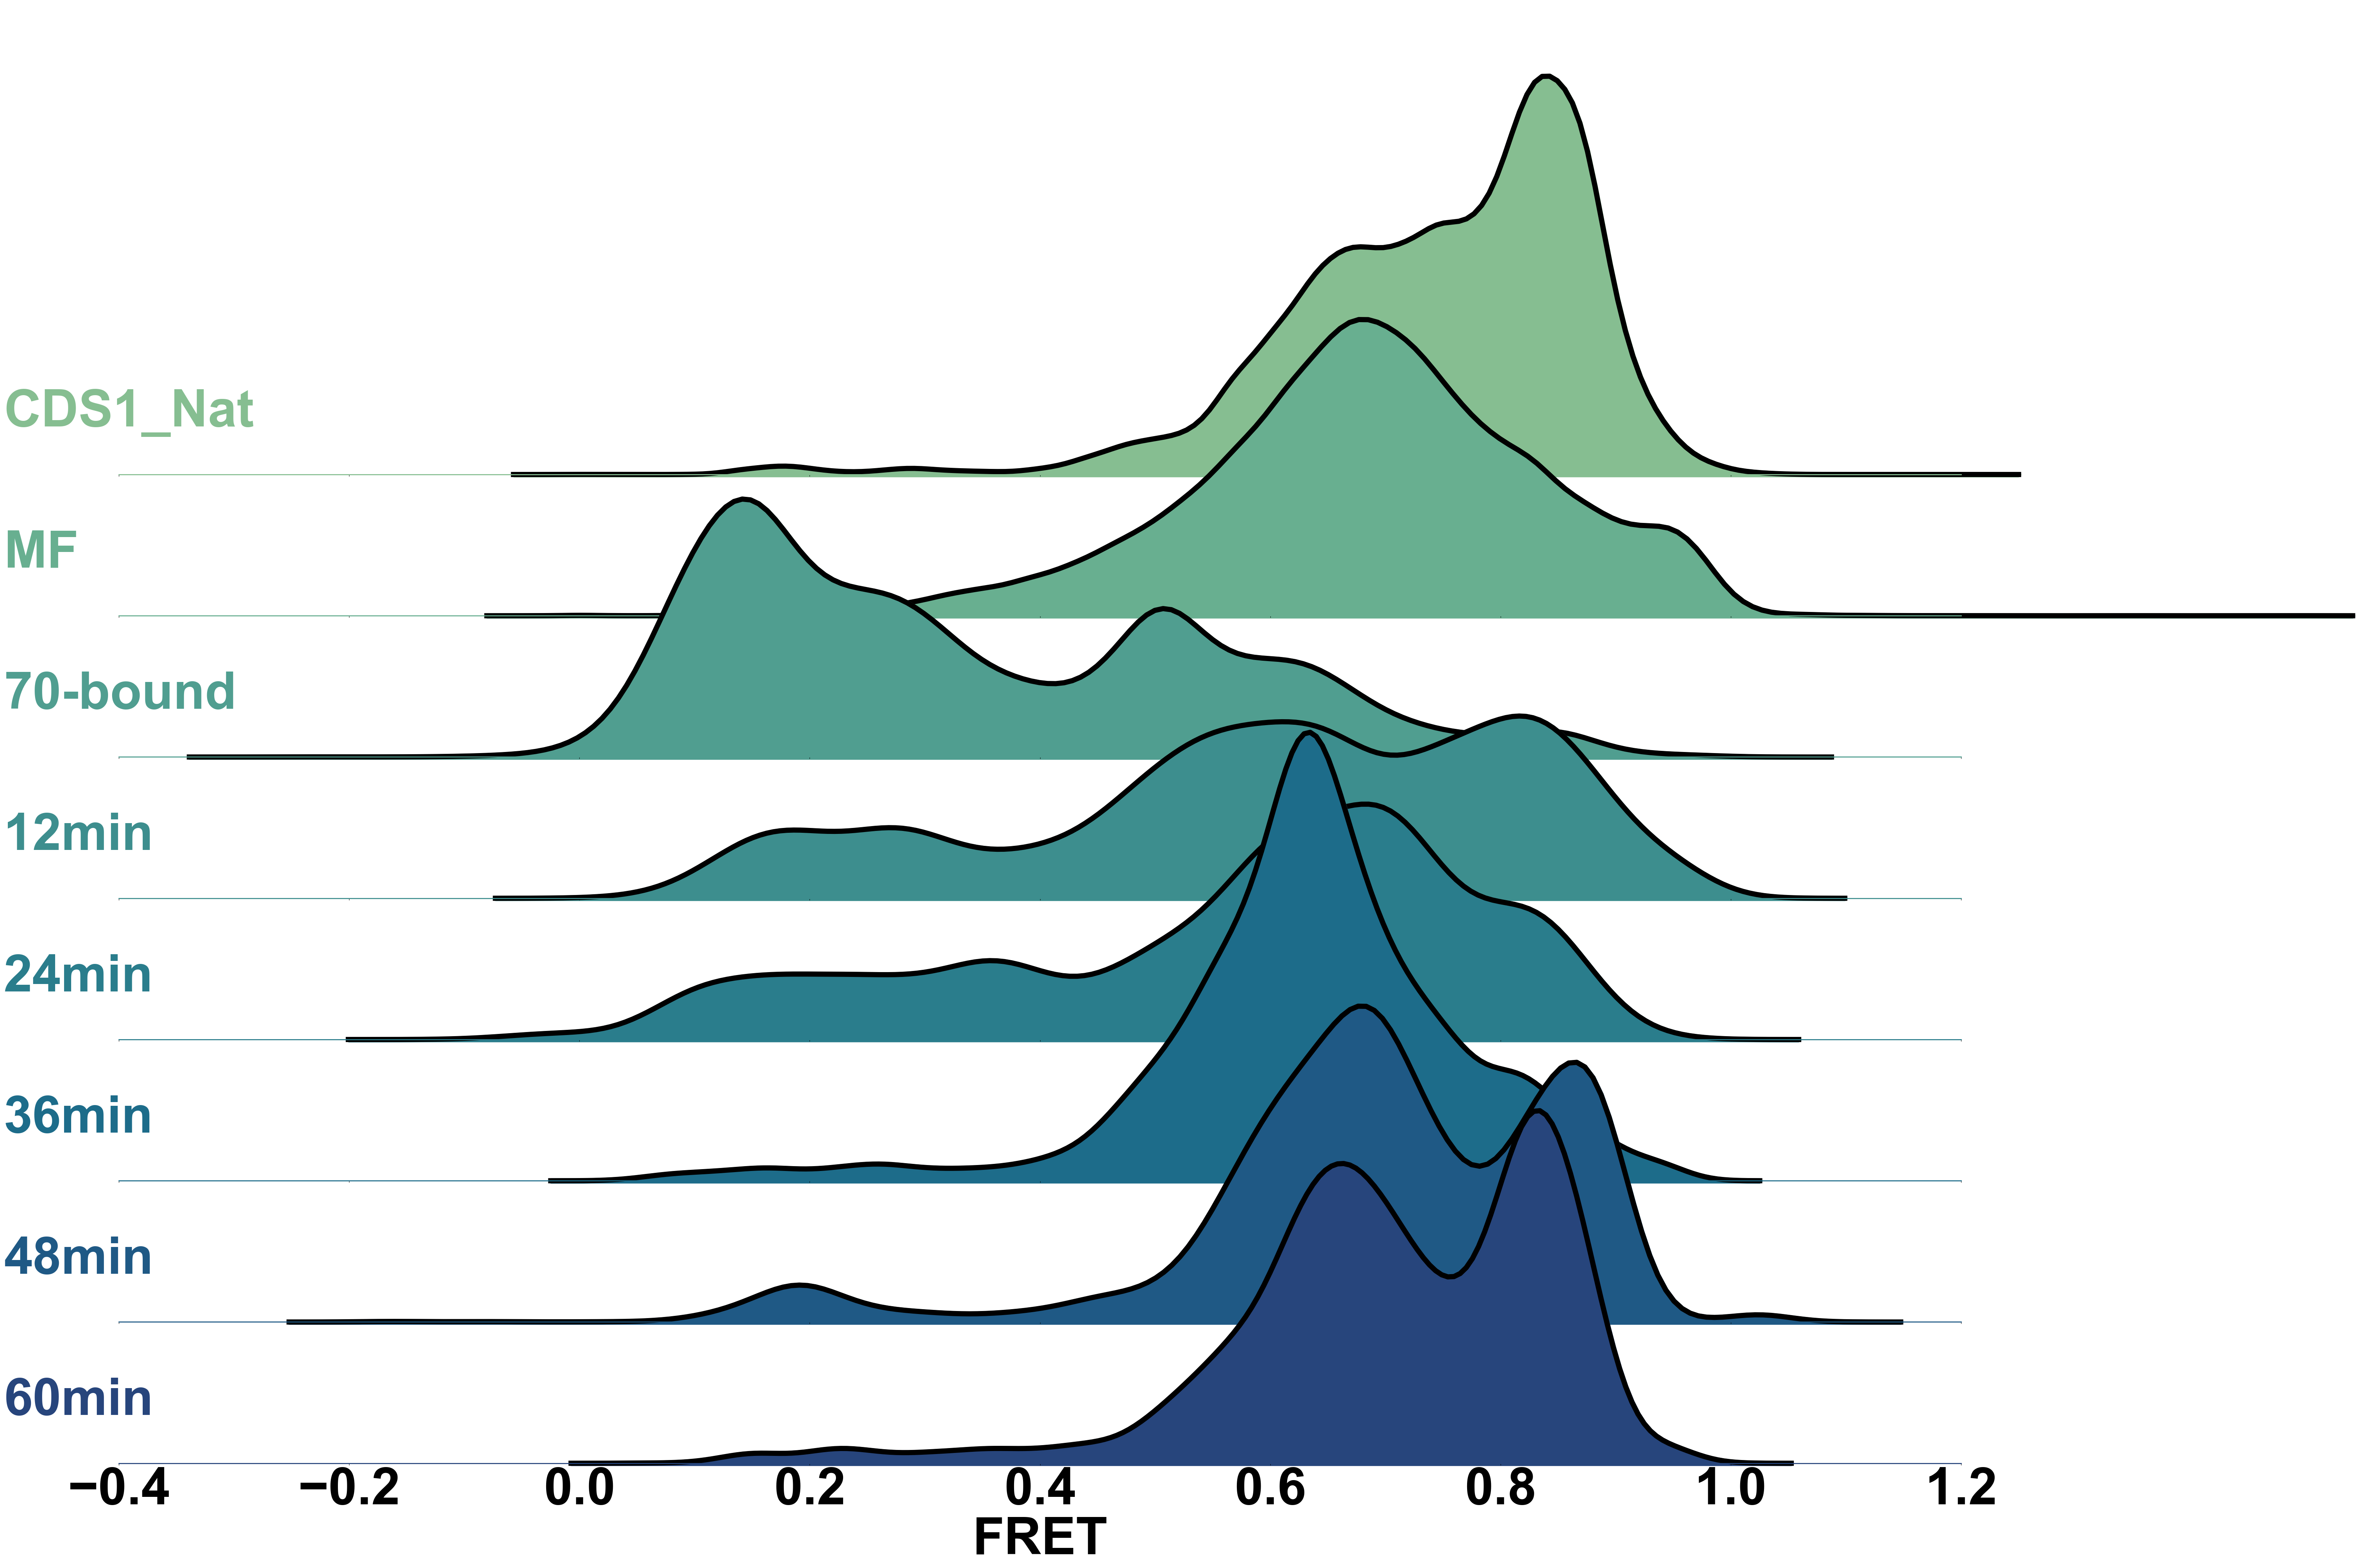
\includegraphics{Hist.png}

\begin{itemize}
\tightlist
\item
  Again I got a strange 70-bound state which doesn't really appear to be
  fully captured by the chaperones.
\item
  Interestingly I get a very prominent 0.6 peak at 36 minutes, but a
  split peak at 60 minutes this time.
\end{itemize}

The previous repeat for this mutant is shown below.

\begin{figure}

{\centering 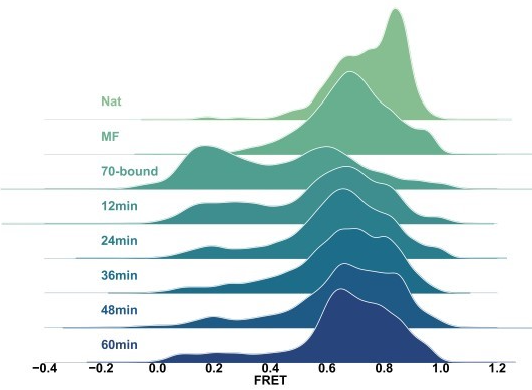
\includegraphics{Capture.PNG}

}

\caption{First real repeat of CDS1}

\end{figure}

\begin{itemize}
\tightlist
\item
  I think I'll wait for the final repeat before starting to collate
  data.
\item
  I also want to refold my sample for an hour with chaperones and then
  flow out chaperones to see what state the fluc exists in following
  refolding once chaperones are removed. Does it prefer the 0.6 or 0.8
  conformation?
\end{itemize}



\end{document}
